\section{Modello XY}

Il modello XY è costituito da un reticolo di spin, i quali presentano due componenti e possono assuemere tutte le orientazioni 
possibili su un piano. Ad ogni posizione reticolare $i$ è associato un angolo $\theta_i$, in modo tale che lo spin ivi giacente 
sia rappresentabile come 

\begin{equation}
    \vec{s_i}\,=\,\left(\sin{\theta_i},\,\cos{\theta_i}\right)
    \label{eq: spin_XY}
\end{equation}

L'hamiltoniana è analoga a quelle considerate in precedenza, caratterizzata da interazione fra primi vicini, con la differenza che 
al posto di una semplice moltiplicazione fra i valori numerici dei due spin ora è presente un prodotto scalare. Si ha quindi che 

\begin{equation}
    H\,=\,-J\sum_{\left<i,j\right>}\vec{s_i} \cdot \vec{s_j}\,-\,\sum_i \vec{h} \cdot \vec{s_i}\,=\,-J\sum_{\left<i,j\right>}\cos{\left(\theta_i\,-\,\theta_j\right)}\,-\,\sum_i \vec{h} \cdot \vec{s_i}. 
    \label{eq: ham_XY}
\end{equation}

Il ground state di questo sistema è caratterizzato da spin totalmente allinati fra loro. In Figura \ref{fig: modelloXY_gs} tale allineamento 
è lungo la verticale, ma in realtà basta che gli angoli relativi fra spin primi vicini siano tutti zero.

\begin{figure}[H]
    \centering
    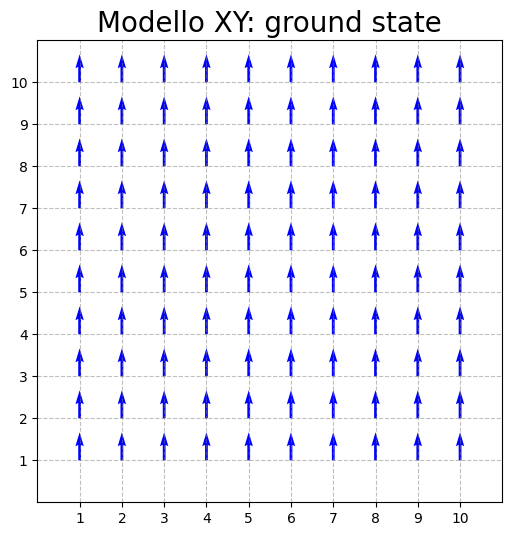
\includegraphics[width=0.5\textwidth]{Immagini/modelloXY_gs.png}
    \caption{Esempio di ground state del modello XY.}
    \label{fig: modelloXY_gs}
\end{figure}





\subsection{Teorema di Mermin-Wigner}

\begin{theorem}[Mermin-Wigner]
    Una simmetria continua non può essere rotta spontaneamente a temperatura finita per sistemi caratterizzati da 
    interazioni a corto raggio e dimensione $d\,\leq\,2$
\end{theorem}

Per avere rottura spontanea di simmetria è necessaria l'assenza del campo magnetico, con conseguente scomparsa del secondo termine 
costituente l'hamiltoniana. Tale quantità gode di simmetria per rotazione di tutti gli spin dello stesso angolo, che è continua, 
in quanto l'angolo di rotazione è un parametro continuo.

Supponendo di porre il sistema nel limite di bassa temperatura, i primi vicini sarebbero fra loro quasi 
paralleli, il che renderebbe $\theta_i\,-\,\theta_j \ll 1$ e di conseguenza consentirebbe l'espansione secondo Taylor della funzione 
coseno. In questo caso l'hamiltoniana risulta 

\begin{equation}
    H\,\simeq\,-J\sum_{\left<i<j\right>}\left[1\,-\,\frac{1}{2}\left(\theta_i\,-\,\theta_j\right)^2\right] = E_0\,+\,\frac{J}{2}\sum_{\left<i<j\right>}\left(\theta_i\,-\,\theta_j\right)^2,  
    \label{eq: ham_XY_app}
\end{equation}

ossia quadratica nella differenza fra coordinate angolari. Dato che è necessario lavorare nel limite termodinamico e che le variazioni 
angolari sono dolci, è possibile passare dal discreto al continuo e lavorare non più in termini di sommatorie, ma in termini di integrali.
la variabile angolare è ora una funzione continua della posizione spaziale $\theta\left(\vec{r}\right)$, in modo che questo ci consenta di 
esplicitare in modo differente il termine quadratico ad argomento della sommatoria precedente \eqref{eq: ham_XY_app}. Infatti è 
possibile riscrivere il tutto come

\begin{equation}
    \mathcal{H} \approx \frac{J_{xy}}{2} \sum_{\langle i<j \rangle} \left( \vartheta_i - \vartheta_j \right)^2 = \frac{J_{xy}}{2} \sum_{\mathbf{r}} \left[ \vartheta (\mathbf{r} + \Delta \mathbf{x}) - \vartheta (\mathbf{r}) \right]^2 
    + \left[ \vartheta (\mathbf{r} + \Delta \mathbf{y}) - \vartheta (\mathbf{r}) \right]^2 = 
    \label{eq: ham_XY_SW}
\end{equation}

\begin{equation*}
    \approx \frac{J_{xy}}{2} \sum_{\mathbf{r}} \Delta x^2 \left[ \frac{\Delta_x \vartheta (\mathbf{r})}{\Delta x} \right]^2 + 
    \Delta y^2 \left[ \frac{\Delta_y \vartheta (\mathbf{r})}{\Delta y} \right]^2 = \\ \frac{J_{xy}}{2} \sum_{\mathbf{r}} \Delta x 
    \Delta y  \left\{ \left[ \frac{\Delta_x \vartheta (\mathbf{r})}{\Delta x} \right]^2 + \left[ \frac{\Delta_y \vartheta 
    (\mathbf{r})}{\Delta y} \right]^2 \right\},
\end{equation*}

dove all'ultimo passaggio abbiamo struttato che $|\Delta \mathbf{x}| = |\Delta \mathbf{y}|$. L'hamiltoniana di partenza \eqref{eq: ham_XY} 
è ora ridotta, in approssimazione di spin wave, a 

\begin{equation}
    H_{SW}\,=\,\frac{J}{2}\int d\vec{r} \left[\nabla \theta \left(\vec{r}\right)\right]^2.
    \label{eq: ham_XY_SW}
\end{equation}

Per valutare quali siano le configurazioni stabili in approssimazione di spin-wave è necessario studiare la variazione 
dell'hamiltoniana, che è possibile dimostrare essere nulla nel momento in cui 

\begin{equation}
    \nabla^2 \theta \left(\vec{r}\right)\,=\,0, 
    \label{eq: LE}
\end{equation}

ossia se la variabile angolare rispetta l'equazione di Laplace. Per risolvere in modo univoco e rigoroso l'equazione precedente è 
necessario specificare delle condizioni al contorno. Lavoriamo ora nel caso di un sistema che ha dimensione lineare L per il quale 

\begin{equation}
    \begin{cases}
        \theta\left(x=0,\,y\right)\,=\,0
        \theta\left(x=L,\,y\right)\,=\,\theta_0
    \end{cases}
    \label{eq: cont_LE}
\end{equation}

La soluzione corretta, riportata in Figura \ref{fig: modelloXY_sw} è qualla di uno stato in cui gli spin sono ruotati di un angolo che dipende dall'ascissa del sito reticolare. 

\begin{figure}[H]
    \centering
    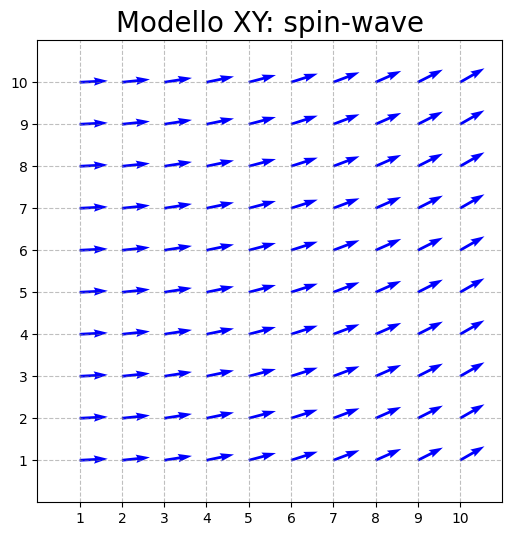
\includegraphics[width=0.5\textwidth]{Immagini/modelloXY_sw.png}
    \caption{Esempio di stato che minimizza la variazione dell'hamiltoniana di spin-wave.}
    \label{fig: modelloXY_sw}
\end{figure}

Dato che 

\begin{equation}
    \theta\left(x,\,y\right)\,=\,\frac{\theta_0}{L}x, 
\end{equation}

sostituendo nell'equazione precedente è possibile apprezzare come 

\begin{equation}
    E = \frac{J}{2} \int d\mathbf{r} \left[ \nabla \vartheta (\mathbf{r}) \right]^2 = \frac{J}{2} \left( \frac{\vartheta_0}{L} \right)^2 L^d = \frac{J}{2} \vartheta_0^2 L^{d-2}
    \label{eq: en_XY_SW}
\end{equation}

Notiamo ora due possibili comportamenti all'aumentare della dimensione lineare $L$ del sistema. Si ha infatti che se 

\begin{itemize}[label=$\diamond$] 
    \item $d\,>\,2$ l'energia aumenta indefinitamente per $L \to \infty$. Questo rende evidente come il sistema è robusto al cambio 
    di condizioni al contorno, poichè è necessaria un'energia al limite infinita per ruotare di un angolo finito entrambi i lati del sistema. 
    In questo caso, il reticolo presenta ordine a lungo raggio.
    \item $d\,<\,2$ l'energia diminusce all'aumentare di $L$, il che rende evidente come il sistema non possa ordinarsi
\end{itemize}

E' possibile dimostrare come il sistema preso in considerazione non presenti ordine a lungo raggio anche per $d\,=\,2$, tuttavia il 
modello XY bidimensionale è comunque caratterizzato da una particolare transizione di fase, che verrà investigata in una delle 
prossime sezioni. 





\subsection{Difetti del parametro d'ordine}

Sebbene l'energia di un certo stato sia minimizzata quando la simmetria è rotta uniformemente in tutto il dominio, tuttavia è possibile 
che tale rottura avvenga in modo differente in parti diverse del campione in analisi. In questi casi emergeranno difetti del parametro d'ordine, 
dovuti all'incompatibilità fra gli ordini locali. Nel caso del modello XY è possibile che si presentino difetti topologici, come per esempio 
i vortici. In Figura \ref{fig: vort_XY} è riportato un esempio di vortice, in cui è possibile apprezzare come al centro dello stesso sia 
presente una singolarità.

\begin{figure}[H]
    \centering
    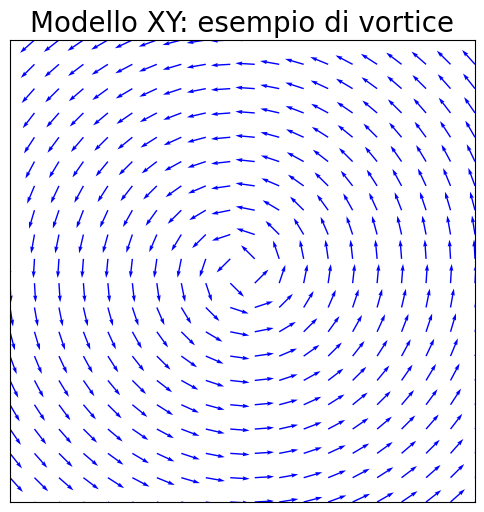
\includegraphics[width=0.5\textwidth]{Immagini/vort_XY.png}
    \caption{Esempio di vortice di spin nel modello XY.}
    \label{fig: vort_XY}
\end{figure}

Tali strutture sono caratterizzate da un \textit{winding number} diverso da zero e non possono rilassarsi autonomamente in modo 
da tornare al ground state. Questo accade perchè la singolarità per essere risolta necessità di un riallineamento dei gradi di libertà 
degli spin. In particolare, la configurazione senza difetti e quella con il vortice non appartengono alla stessa classe d'omotopia, 
e quindi non è possibile deformare con continuità l'una nell'altra. Questo è evidente in Figura \ref{fig: homCl_XY}, 
che sulla prima riga presenta delle configurazioni a winding number nullo, mentre sulla seconda a winding number pari ad uno. Accanto agli spin è 
presente una raffigurazione dello spazio del parametro d'ordine, il quale viene percorso facendo un giro completo nel caso dei difetti (c) e (d). 

\begin{figure}[H]
    \centering
    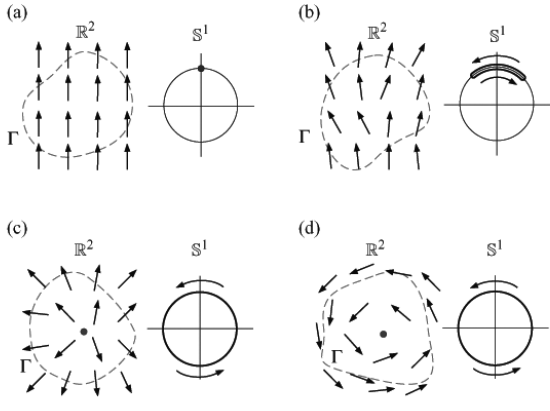
\includegraphics[width=0.7\textwidth]{Immagini/homCl_XY.png}
    \caption{Confronto fra configurazioni appartenenti a diverse classi d'omotopia. Alla prima riga le strutture riportate hanno winding 
    number pari a zero, e questo è evidenziato da come sia esplorato solo localmente lo spazio del parametro d'ordine. Alla seconda riga sono 
    invece riportate le configurazioni (c) e (d), entrambe con winding number pari ad uno, che si traduce in un'esplorazione completa di tutte le 
    possibili orientazioni del parametro d'ordine. Immagine da \cite{galliFSA}.}
    \label{fig: homCl_XY}
\end{figure}


\subsection{Transizione Kosterlitz-Thouless}
